
%-------------------------------------------------------------------------------
\chapter{Análise do Problema}
\label{sec:AP}

Neste próximo capítulo aborda-se a análise do problema em questão. Inicia-se com a descrição do domínio do problema, através do glossário de termos usados, do modelo de domínio e do mapa de materialidade da Devscope de acordo com as métricas indicadas pela \gls{SASB} para o setor de \textit{software} e serviços IT. Por fim, serão delineados os requisitos funcionais e não funcionais do sistema.

\section{Contexto}
\label{sec:Context}

A fase de análise é uma das mais importantes no ciclo de vida do desenvolvimento de software, pois é nela que ocorre a recolha dos requisitos, funcionalidades e necessidades do cliente, bem como das especificações do sistema. O objetivo final é definir de forma clara os recursos e funcionalidades que compõem a solução a ser desenvolvida.

Qualquer informação incorreta ou não obtida pode comprometer o desenvolvimento do produto, tanto em termos de qualidade como de cumprimento dos prazos.

A proposta de desenvolvimento de uma plataforma ESG surgiu da necessidade identificada pela Devscope em centralizar e otimizar o controlo de diversas métricas relacionadas com os pilares ambiental, social e de governança (ESG). Esta necessidade prende-se com a crescente importância de monitorizar e reportar práticas sustentáveis, promovendo uma gestão mais transparente, eficiente e alinhada com os objetivos de responsabilidade corporativa da empresa. Ao centralizar estes dados numa única plataforma, a Devscope pretende não só melhorar a sua capacidade de análise e tomada de decisões, como também reforçar o seu compromisso com a sustentabilidade e o impacto positivo na sociedade.

\section{Domínio do problema}
\label{sec:DP} 
% Devem ser especificados os conceitos de domínio do problema através de artefactos adequados (e.g. glossário, modelo de domínio). 

A presente secção visa descrever o domínio do problema através de vários artefactos de variadas complexidades, nomeadamente conceitos e diagramas.

A Tabela \ref{tab:glossario_dominio} apresenta os conceitos introduzidos no domínio do problema e que serão usados ao longo do desenvolvimento.

%- Glossario da soluçao (termos usados ao longo do desenvolvimento e o que são)
\begin{table}[H]
    \rowcolors{2}{purple!10}{white}
    \renewcommand{\arraystretch}{1.2}
    \setlength{\tabcolsep}{10pt}
    \centering
    \begin{tabular}{>{\bfseries}p{3.5cm} >{\bfseries}p{4cm} p{7cm}}
        \rowcolor{purple!40}
        Conceito (EN) & Conceito (PT) & \textbf{Descrição} \\
        ESG & ESG (Ambiente, Social, Governança) & Conjunto de critérios que avaliam o desempenho ambiental, social e de governança de uma organização, com foco na sustentabilidade e responsabilidade corporativa. \\
        Dashboard & Painel & Resumo gráfico de várias informações importantes, normalmente utilizado para dar uma visão geral de um negócio. \\
        Materiality Map & Mapa de Materialidade & Ferramenta que destaca as métricas ESG mais relevantes para cada setor, segundo as normas da SASB. \\
        % Podes adicionar mais linhas abaixo
    \end{tabular}
    \caption{Glossário do domínio do problema}
    \label{tab:glossario_dominio}
\end{table}

A Figura \ref{fig:domain_model} ilustra o modelo de domínio e relaciona os diferentes conceitos da solução.

% - Modelo de dominio (diagrama)
\begin{figure}[h]
    \centering
    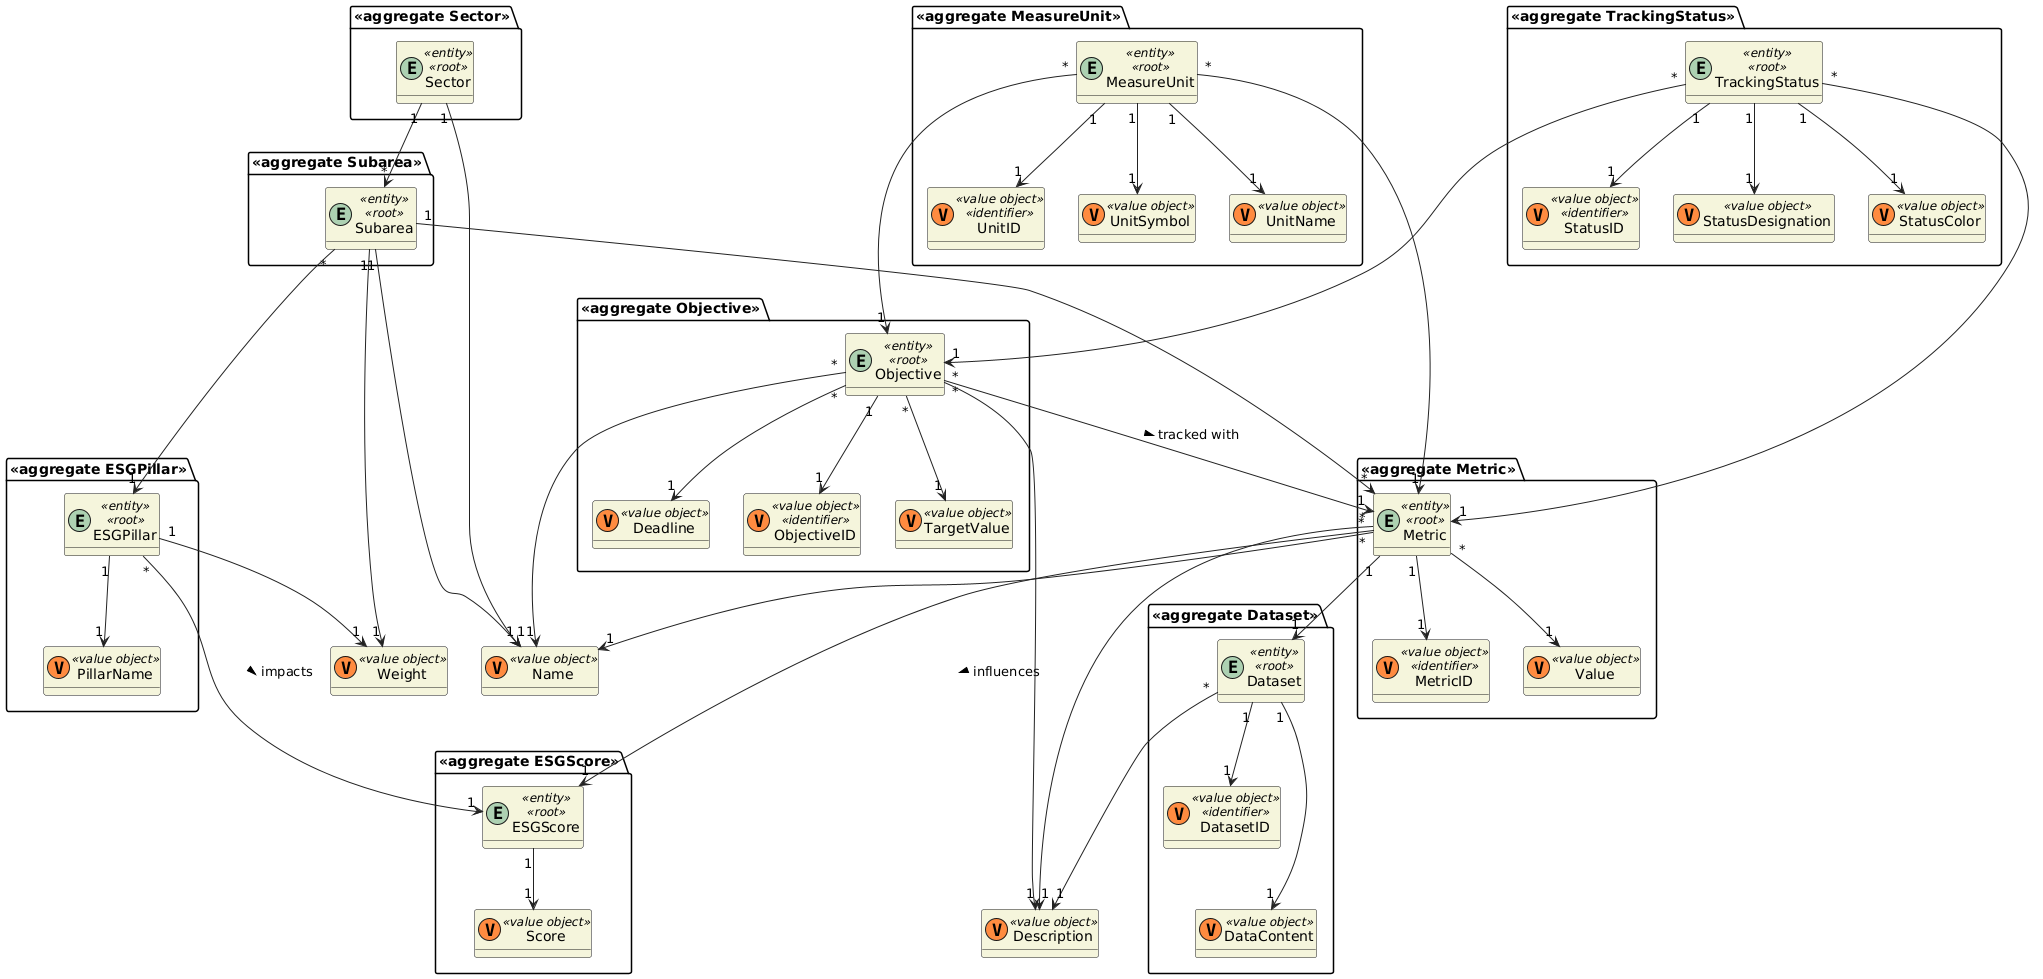
\includegraphics[width=\linewidth,keepaspectratio]{frontmatter/assets/diagrams/Domain Model/Domain_Model.png}
    \caption{Modelo de Dominio}
    \label{fig:domain_model}
\end{figure}

O \textit{dashboard} apresenta a pontuação ESG da empresa com base na consolidação de todas as métricas contabilizadas, permitindo uma visão geral do desempenho. Além disso, destaca o desempenho das principais métricas, bem como aquelas que melhoraram ou pioraram ao longo da semana, com a possibilidade de visualizar também o histórico mensal e anual dessas métricas.

Outra seção da plataforma disponibiliza uma visão detalhada de todas as métricas existentes: métricas alinhadas com os \gls{ODS}, métricas personalizadas (criadas pelos próprios utilizadores) e métricas orientadas pelos padrões definidos pela \gls{SASB}.

Cada métrica possui atributos específicos, incluindo o pilar e subárea ESG a que pertence, o seu nível de influência na pontuação ESG, unidade de medida, código identificador e os dados importados que lhe estão associados.

De acordo com o referencial \gls{SASB}, adotado pela Devscope, existem normas específicas para cada setor — como é o caso do setor de Software e Serviços de TI — que determinam quais métricas devem ser reportadas (\cite{SASBSector2025}). É com base nessas diretrizes que se constrói o Mapa de Materialidade, como indicado na Figura \ref{fig:materiality_map}.

Este mapa, um dos elementos centrais da plataforma, reflete as métricas ativas não só definidas pela \gls{SASB}, consoante o setor da empresa, bem como as métricas personalizadas. Este mapa organiza as métricas segundo os pilares ESG e respectivas subáreas, proporcionando uma visão estruturada das prioridades de sustentabilidade da organização.

% - mapa de materialidade da DevScope (Software e IT sector - SASB)
\begin{figure}[h]
    \centering
    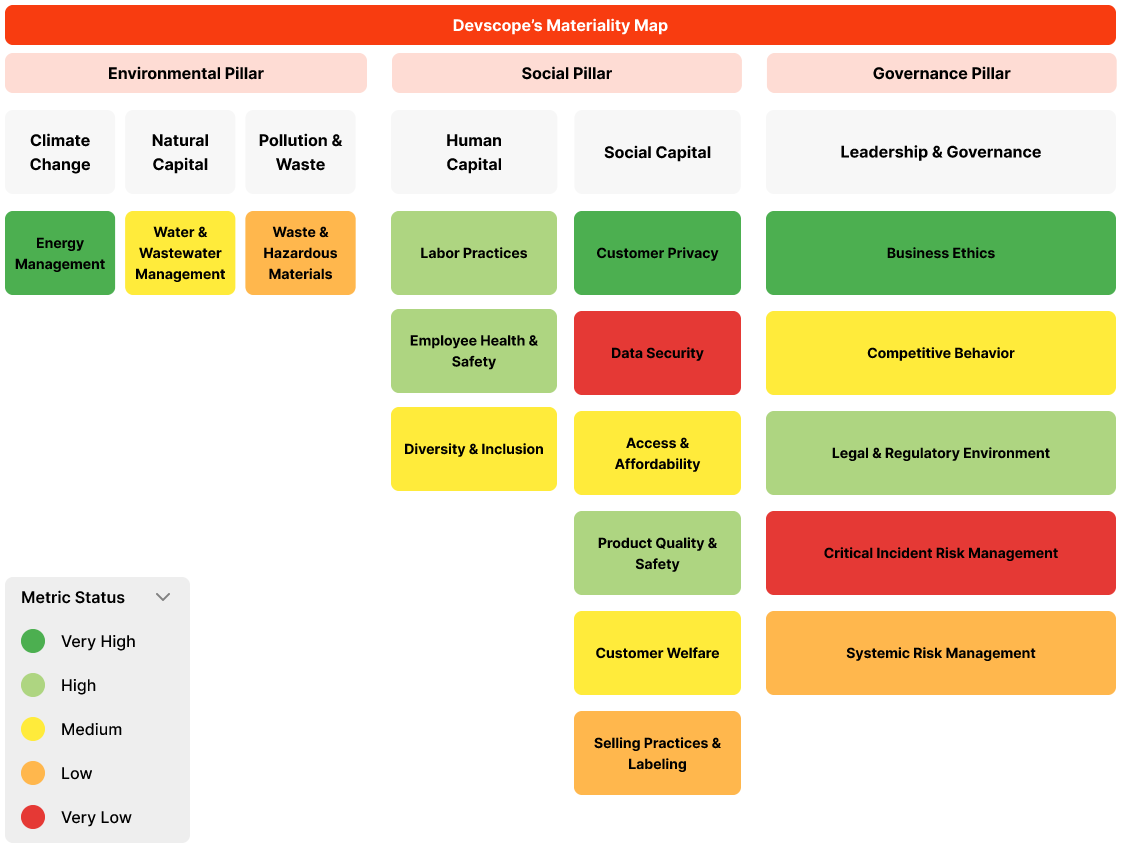
\includegraphics[width=\linewidth]{frontmatter/assets/mapa-materialidade.png}
    \caption{Mapa de Materialidade segundo o setor SASB da Devscope (Software e serviços IT)}
    \label{fig:materiality_map}
\end{figure}

Por fim, outra página da plataforma é dedicada à gestão de objetivos, permitindo acompanhar os objetivos definidos, as métricas a eles associadas, o progresso na sua concretização e, semanalmente, se se encontram dentro ou fora do plano estabelecido.

\section{Requisitos funcionais e não funcionais}

A seguinte seção compila os requisitos obtidos com o cliente e categoriza-os entre funcionais e não funcionais.

\subsection{Requisitos Funcionais}

Os requisitos funcionais correspondem a funcionalidades presentes no software a ser desenvolvido, normalmente representadas por casos de uso e acompanhados por diagramas. Os requisitos funcionais deste projeto estão organizados na Tabela \ref{tab:use_cases}, onde cada requisitos é considerado um caso de uso e identificado por um código alfa-numérico.

%- Use Cases list
\begin{table}[H]
    \rowcolors{2}{orange!20}{white}
    \renewcommand{\arraystretch}{1.2}
    \setlength{\tabcolsep}{10pt}
    \centering
    \begin{tabular}{>{\bfseries}p{3.5cm} p{4cm} p{7cm}}
        \rowcolor{orange!50}
        Código & \textbf{Descrição Curta} & \textbf{Descrição} \\
        UC-01 & Visualização de KPI's & Como analista ESG, quero visualizar rapidamente os principais KPIs ambientais, sociais e de governação, para poder avaliar o desempenho da organização. \\
        UC-02 & Filtragem de Métricas & Como stakeholder, quero poder filtrar os dados por setor e ano, para analisar tendências específicas ao longo do tempo. \\
        UC-03 & Mapa de Materialidade & Como colaborador da área de sustentabilidade, quero ver a mapa de materialidade para priorizar temas relevantes com base no setor. \\
        UC-04 & Pontuação ESG & Como gestor, quero aceder a uma pontuação ESG agregada, para ter uma visão geral do desempenho da empresa em responsabilidade social e ambiental. \\
        UC-05 & Detalhes de Métricas & Como utilizador curioso, quero clicar num KPI e ver mais detalhes históricos e explicações, para compreender o que influencia cada indicador. \\
        UC-06 & Mapa de Materialidade Detalhada & Como utilizador analítico, quero visualizar a matriz de materialidade dividida por categorias ESG com um sistema de cores intuitivo, para identificar rapidamente os temas mais críticos e, ao clicar em cada indicador, aceder a detalhes explicativos que me ajudem a compreender o seu impacto e evolução. \\
        UC-07 & Métricas Customizáveis & Como gestor de sustentabilidade, quero poder criar métricas ESG específicas à realidade da empresa e definir a sua fonte de dados, para garantir que o painel reflete os indicadores mais relevantes para a nossa estratégia. \\
        UC-08 & Importe de Dados & Como gestor de sustentabilidade, quero poder importar dados para associar às métricas. \\
        UC-09 & Modo Noturno & Como utilizador, quero poder alternar entre modo noturno e modo claro \\        
    \end{tabular}
    \caption{Lista de Casos de Uso}
    \label{tab:use_cases}
\end{table}

De modo a melhorar a leitura do documento, os diagramas da vista de processos, segundo o modelo de vistas arquiteturais concorrentes 4+1 (\cite{Kruchten1995}), serão apresentados em conjunto com a análise de cada caso de uso. Todas as outras vistas serão exploradas no próximo capitulo \ref{sec:DP}.

\subsubsection{UC-01 | Visualização de KPI's}

% 1. Como analista ESG, quero visualizar rapidamente os principais KPIs ambientais, sociais e de governação, para poder avaliar o desempenho da organização.
% %     ○ Visualização rápida de métricas chave (emissões, diversidade, etc.)
% %     ○ Divididos por categorias: Ambiental, Social e Governança

\subsubsection{UC-02 | Filtragem de Métricas}

% % 2. Como analista ESG, quero poder filtrar os dados por setor e ano, para analisar tendências específicas ao longo do tempo.
% %     ○ Ano / intervalo temporal
% %     ○ Categoria ESG (filtrar por E, S ou G)

\subsubsection{UC-03 | Mapa de Materialidade}

% % 5. Como analista ESG, quero ver a matriz de materialidade para priorizar temas relevantes com base no setor.
% %     ○ Representação visual dos temas ESG mais relevantes para o setor
% %     ○ Com base no modelo SASB (Software & IT)
% %     ○ Permite identificar prioridades estratégicas (talvez com recomendações ??)

\subsubsection{UC-04 | Pontuação ESG}

% % 4. Como analista ESG, quero aceder a uma pontuação ESG agregada, para ter uma visão geral do desempenho da empresa em responsabilidade social e ambiental.
% %     ○ Atribuição de uma "pontuação ESG" global (ex: 0–100, A–F, etc.) - depois explorar isto
% %     ○ Visualização por medidores ou cores

\subsubsection{UC-05 | Detalhes de Métricas}

% % 3. Como analista ESG, quero clicar num KPI e ver mais detalhes históricos e explicações, para compreender o que influencia cada indicador.
% %     ○ Permitir clicar nos KPIs ou gráficos para ver mais detalhes
% %     ○ Informação histórica, iniciativas associadas, notas explicativas

\subsubsection{UC-06 | Mapa de Materialidade Detalhada}

% 6. Como analista ESG, quero visualizar a matriz de materialidade dividida por categorias ESG com um sistema de cores intuitivo, para identificar rapidamente os temas mais críticos e, ao clicar em cada indicador, aceder a detalhes explicativos que me ajudem a compreender o seu impacto e evolução.

\subsubsection{UC-07 | Métricas Customizáveis}

% 7. Como analista ESG, quero poder criar métricas ESG específicas à realidade da empresa e definir a sua fonte de dados, para garantir que o painel reflete os indicadores mais relevantes para a nossa estratégia.

\subsubsection{UC-08 | Importe de Dados}

\subsubsection{UC-09 | Modo Noturno}


\subsection{Requisitos Não Funcionais}

Requisitos não funcionais correspondem a todas as outras propriedades que não constituem funcionalidades, como performance, usabilidade, uso de tecnologias ou processos específicos, entre outras restrições/limitações na solução desenvolvida.

Uma forma de categorizar os requisitos não funcionais  é através de FURPS +.
(Explicar o que cada letra quer dizer)

- explicar conceito de FURPS+
- apresentar e categorizar os requisitos não funcionais conforme FURPS+

- Modo escuro e modo claro
- Fonte de dados simulada
- SASB

%-------------------------------------------------------------------------------

\chapter{Desenho da solução}
Breve introdução sobre o capitulo

//indicate whats supposed to do in the design phase of design

\section{Arquitetura do Sistema} 

- 4+1 model
- C4 model
- clean arquitecture
- model-view-controller

- views (system, container maybe component if necessary)

say that:
(process views of each US are together with its analysis to be easier to understand and flesh out previous chapter)


\begin{figure}[H]
    \centering
    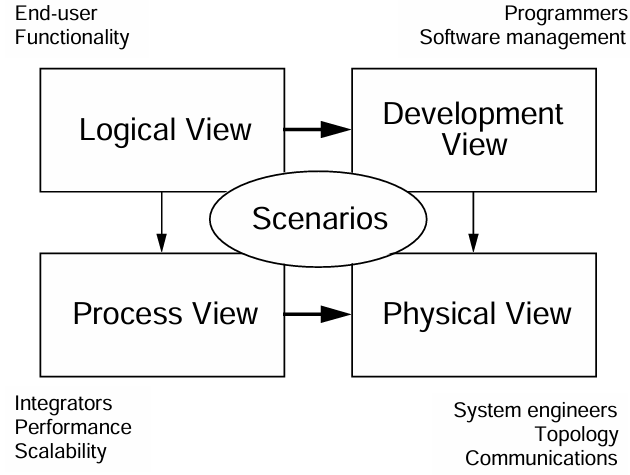
\includegraphics[width=4in,keepaspectratio]{frontmatter/assets/diagrams/4+1views.png}
    \caption{Modelo de Vistas 4+1}
    \label{fig:41viewmodel}
\end{figure}


\begin{figure}[H]
    \centering
    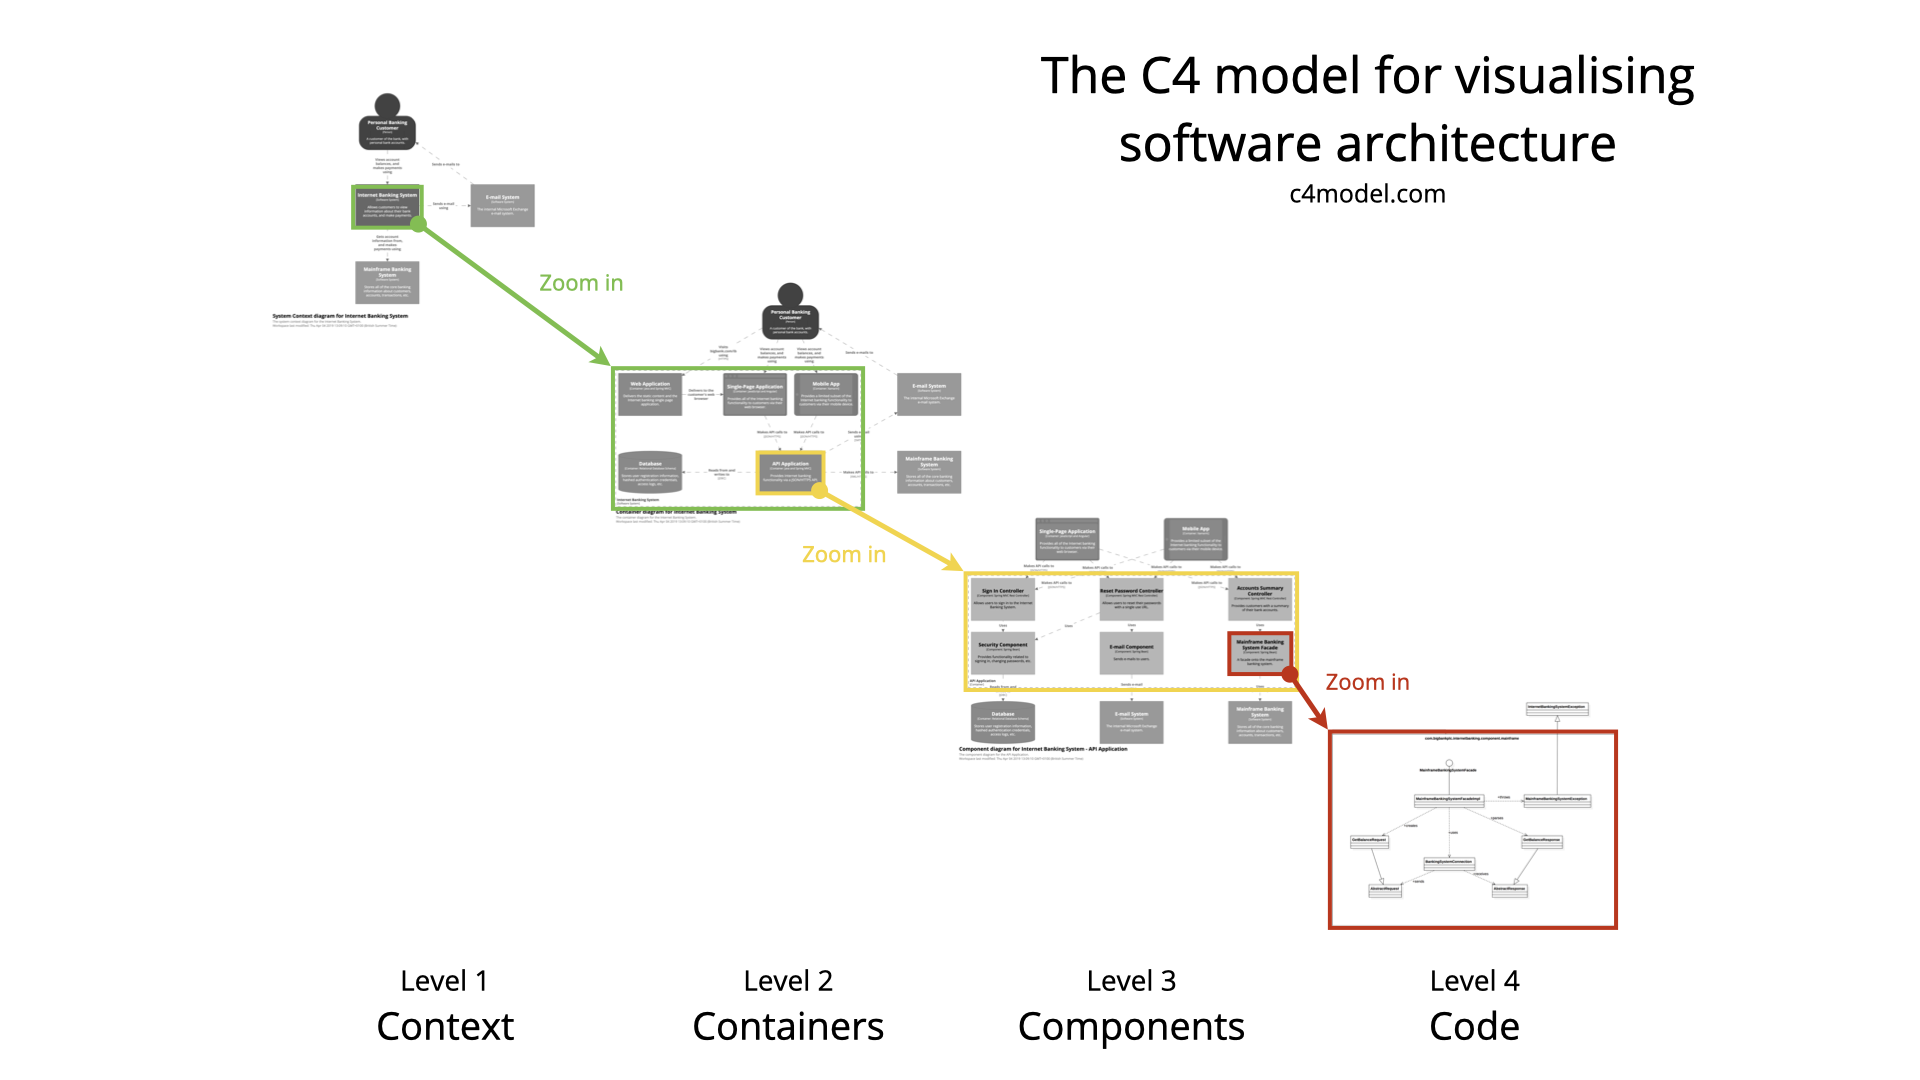
\includegraphics[width=\linewidth,keepaspectratio]{frontmatter/assets/diagrams/c4-overview.png}
    \caption{Modelo Arquitural C4}
    \label{fig:c4model}
\end{figure}


\subsection{Vista de Cenários}

A vista de cenários compila os caso de usos mais gerais, no fundo, sendo uma abstração dos requisitos mais importantes, já explorados no capítulo anterior. Esta vista é vista como redundante, daí o "+1" na designação do modelo arquitetural (\cite{Kruchten1995}). A Figura \ref{fig:scenario_view} ilustra esta vista.

\begin{figure}[H]
    \centering
    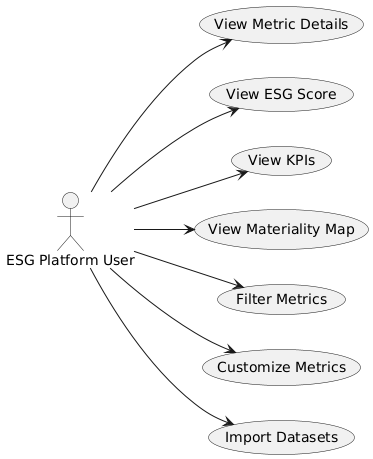
\includegraphics[height=5in,keepaspectratio]{frontmatter/assets/diagrams/Scenario View/Scenario_View.png}
    \caption{Vista de Cenários}
    \label{fig:scenario_view}
\end{figure}

\subsection{Vista Lógica}

A vista lógica tem como objetivo estruturar a arquitetura do sistema com foco nos requisitos funcionais, aquilo que o sistema deve ser capaz de fazer a nivel de serviços para os seus utilizadores, de uma forma mais abstrata, servindo para identificar mecanismos comuns e design de elementos ao longo das várias partes do sistema.

Esta vista será abordada por vários diagramas correspondentes a sucessivos níveis de detalhe na representação logica do sistema, iniciando-se pelo nível 1, com a Figura \ref{fig:logical_view_lv1}.

\begin{figure}[H]
    \centering
    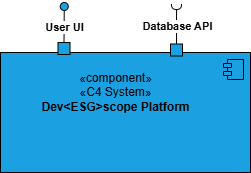
\includegraphics[width=2in,keepaspectratio]{frontmatter/assets/diagrams/Logical View/Logical View Lv1.drawio.png}
    \caption{Vista Lógica Nível 1}
    \label{fig:logical_view_lv1}
\end{figure}



\begin{figure}[H]
    \centering
    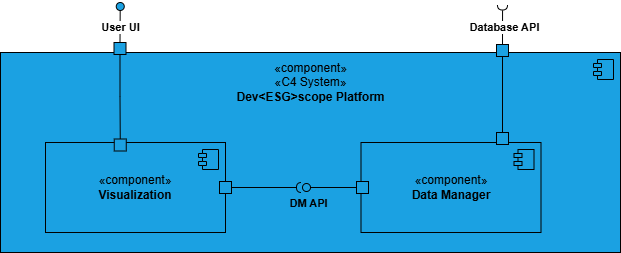
\includegraphics[width=5in,keepaspectratio]{frontmatter/assets/diagrams/Logical View/Logical View Lv2.drawio.png}
    \caption{Vista Lógica Nível 2}
    \label{fig:logical_view_lv2}
\end{figure}


\begin{figure}[H]
    \centering
    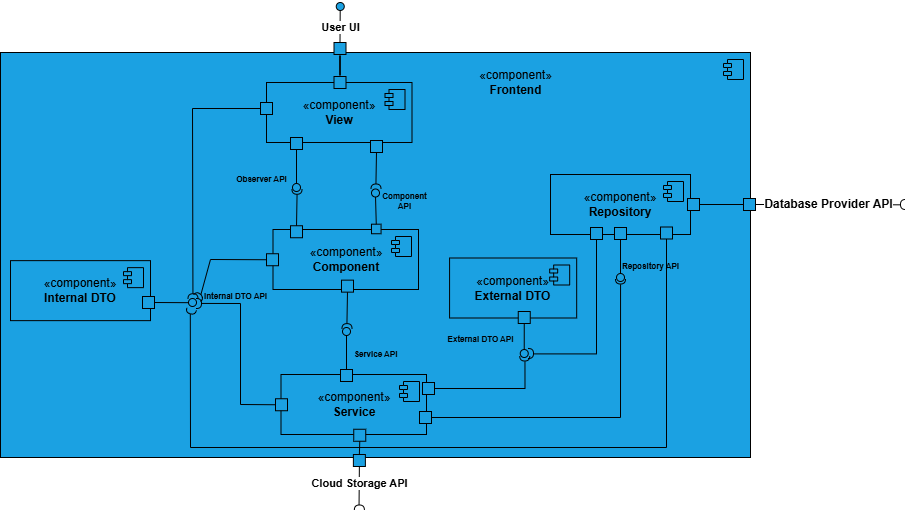
\includegraphics[width=6.5in,keepaspectratio]{frontmatter/assets/diagrams/Logical View/Logical View Lv3.drawio.png}
    \caption{Vista Lógica Nível 3}
    \label{fig:logical_view_lv3}
\end{figure}


- logical (1-3 levels)


\subsection{Vista de Implementação}
- implementation (2 e 3 level)



\begin{figure}[H]
    \centering
    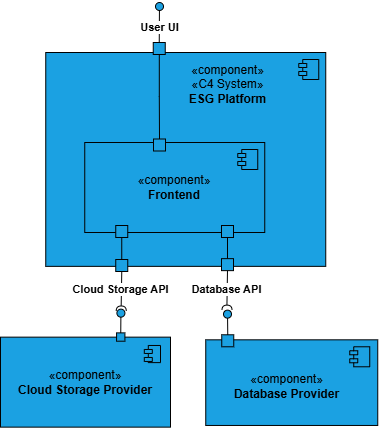
\includegraphics[width=5in,keepaspectratio]{frontmatter/assets/diagrams/Development View/Implementation View Lv2.drawio.png}
    \caption{Vista de Implementação Nível 2}
    \label{fig:development_view_lv2}
\end{figure}


\begin{figure}[H]
    \centering
    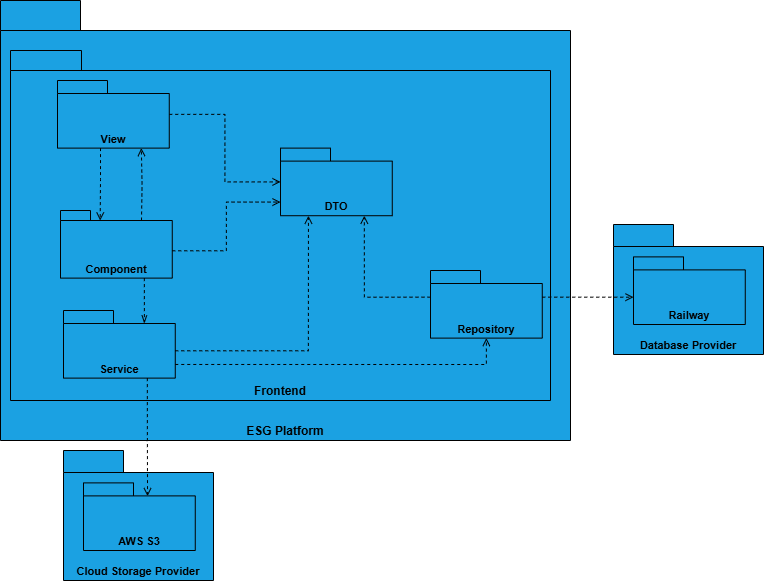
\includegraphics[width=6.5in,keepaspectratio]{frontmatter/assets/diagrams/Development View/Implementation Lv3.drawio.png}
    \caption{Vista de Implementação Nível 3}
    \label{fig:development_view_lv3}
\end{figure}


    
\subsection{Vista Física}

A \textbf{vista física} tem como objetivo mapear o \textit{software} para o \textit{hardware}, com ênfase nos \textbf{requisitos não funcionais} do sistema, como disponibilidade,confiabilidade (tolerância a falhas), desempenho e escalabilidade (\cite{Kruchten1995}). A Figura~\ref{fig:physical_view_lv2} apresenta o diagrama de nível 2 da vista física da solução desenvolvida.


\begin{figure}[H]
    \centering
    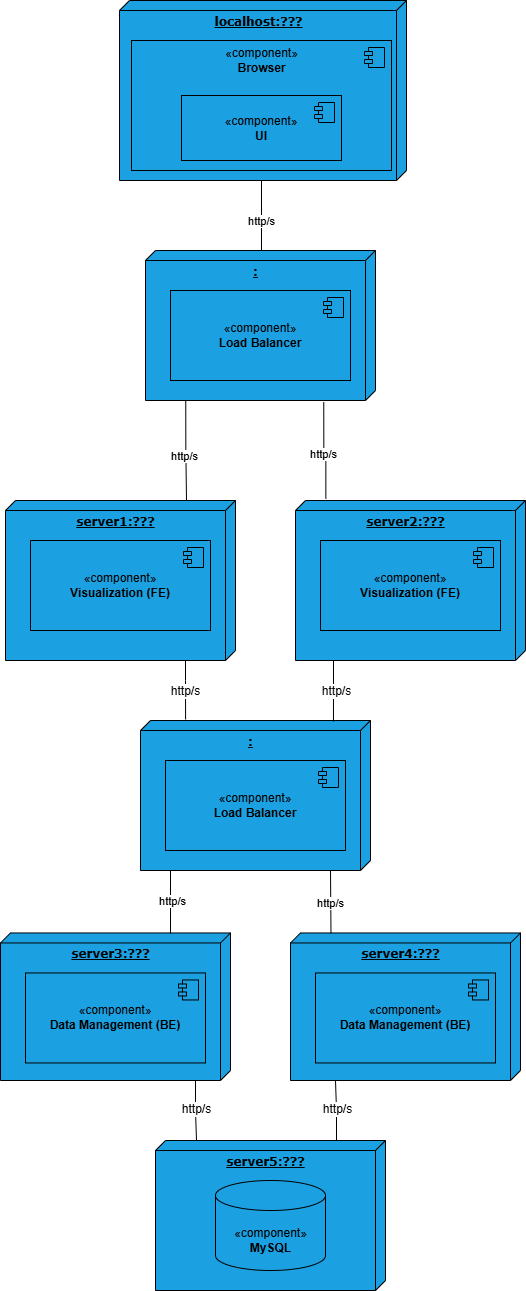
\includegraphics[height=8in,keepaspectratio]{frontmatter/assets/diagrams/Physical View/physical_view_lv2.drawio.png}
    \caption{Diagrama de nível 2 da vista física da solução}
    \label{fig:physical_view_lv2}
\end{figure}


Os \textbf{Load Balancers} são responsáveis por distribuir o tráfego de forma dinâmica entre os servidores que compõem as camadas de \textit{Visualization} (\textit{frontend}) e \textit{Data Management} (\textit{backend} com base de dados). Estes atuam como intermediários entre os utilizadores e os servidores, assegurando uma \textbf{distribuição equilibrada da carga}, especialmente durante períodos de maior tráfego. Com isso, aumentam a disponibilidade e a resiliência do sistema: caso um servidor falhe, o tráfego é automaticamente redirecionado para outro servidor ativo (tolerância a falhas). Esta abordagem contribui ainda para a redução da latência e para evitar respostas inconsistentes da aplicação (\Cite{F52025}).

As comunicações entre os vários componentes são realizadas através de protocolo HTTP ou HTTPS.